\documentclass[smaller,unicode,hyperref={unicode=true}]{beamer}
\mode<presentation> {
  \usetheme{Singapore}
  \useinnertheme{circles}
  \setbeamertemplate{navigation symbols}{}%remove navigation symbols
  % \usecolortheme{whale}
}


\usepackage[russian]{babel}
\usepackage[utf8]{inputenc}
\usepackage{color}
\usepackage{subcaption}

\usepackage{amsmath}
\usepackage{amssymb}
\usepackage{graphics}
\usepackage{epsfig}
% \usepackage{times}

\title{Обзор методов решения задачи MAP}

\author[Новиков]
{А.\,В.~Новиков\inst{1}}
\institute[МГУ ВМК]
{
  \inst{1}
  МГУ, ВМиК, каф. ММП
}

\date[Lecture 1]
{
  Спецсеминар <<Байесовские методы машинного обучения>>
}

\begin{document}

\begin{frame}
  \titlepage
\end{frame}
\begin{frame}
  \frametitle{Оглавление}
\tableofcontents[currentsection]
\end{frame}

\section[Задача]{Постановка задачи}
\begin{frame}
  \frametitle{Постановка задачи}
    \begin{equation*}
        P(x~|~z) \propto \prod_{a \in V} \psi (z_a~|~x_a) \prod_{(a,b) \in E} \psi_{ab} (x_{a}, x_{b}) \rightarrow \max_{X}
    \end{equation*}
    \begin{equation}
        E(x) = \sum_{a \in V} \varphi_a (x_a) + \sum_{(a,b) \in E} \varphi_{ab} (x_{a}, x_{b}) \rightarrow \min_{X}
    \end{equation}

    \begin{figure}
      \includegraphics[scale=0.6]{segmentation.eps}
    \end{figure}
\end{frame}

\section{Алгоритмы}
\begin{frame}
  \frametitle{Обзор алгоритмов}
    \begin{itemize}
      \item Alpha--Expansion
      \item Loopy belief propagation
      \item TRW--S~\cite{TRWS}
      \item Субградиентный подъём~\cite{Subgradient}
      \item Bundle methods~\cite{Bundle}
      \item L--BFGS
      % \item <<Полная декомпозиция>>
  \end{itemize}
\end{frame}

% \section{Обозначения}
% \begin{frame}
%   \frametitle{Обозначения}
%   Марковская случайная сеть задана графом $G$:\\
%     \begin{equation*}
%         G = (V, E)
%     \end{equation*}
%   Переменная прямой задачи обозначается $x_a \in \{1, \dots, K\}$ и индексируется вершиной $a \in V$.
%     \begin{equation*}
%         X = \{x_a\}_{a \in V}
%     \end{equation*}
%     $\theta_{a,p} = \varphi_{a} (p)$, $\theta_{ab,pq} = \varphi_{ab} (p, q)$.\\
%     $\mathcal{M}$ --- исходные ограничения ($y_{a,p}, y_{ab,pq} \in \{0,~1\}$).\\
%     $\mathcal{R}$ --- LP--релаксация ($y_{a,p}, y_{ab,pq} \in [0,~1]$).\\
%     $\mathcal{L}$ --- множество ограничений на лямбду.
%     Граф разбивается на деревья $\{D^t\}_{t=1}^T$.\\
%     $n_a$ --- число деревьев включающих вершину $a$.\\
%     \begin{equation*}
%      E(Y, \Theta) = \sum_{a \in V} \sum_{p = 1}^{K} \theta_{a,p} y_{a,p} + \sum_{(a,b) \in E} \sum_{p,q = 1,1}^{K} \theta_{ab,pq} y_{ab,pq}
%     \end{equation*}
%     $P_C(\cdot)$ используется для обозначения Евклидовой проекции на множество $C$.
% \end{frame}

\section{Частные случаи}
\begin{frame}
  \frametitle{Разрез графов}
  В случае если задача бинарная ($K = 2$) и выполнено <<условие субмодулярности>> ($\varphi_{ab} (0, 0) + \varphi_{ab} (1, 1) \leq \varphi_{ab} (0, 1) + \varphi_{ab} (1, 0)$), то можно применять очень эффективные алгоритмы основанные на разрезе графов.
    \begin{figure}
      \includegraphics[scale=0.35]{graph_cut.eps}
    \end{figure}
\end{frame}
% \begin{frame}
%   \frametitle{Belief propagation}
%   Лалала
% \end{frame}

\section{Двойственное разложение}
\begin{frame}
  \frametitle{Двойственное разложение (пример)}
  Пусть у нас есть задача
  \begin{equation*}
    f(x) + g(x) \rightarrow \min_{x}
  \end{equation*}
  причем задачи
  \begin{align*}
      f(x) \rightarrow \min_{x}\\
      g(x) \rightarrow \min_{x}
  \end{align*}
  мы умеем решать быстро. Тогда:
  \begin{align*}
      f(x_1) + g(x_2) \rightarrow \min_{x_1, x_2}\\
      such~that~x_1~=~x_2
  \end{align*}
  \begin{equation*}
      \max_{\lambda} \min_{x_1, x_2} f(x_1) + g(x_2) + \lambda (x_2 - x_1)
  \end{equation*}
  \begin{equation*}
      \max_{\lambda} \min_{x_1, x_2} f(x_1) - \lambda x_1 + g(x_2) + \lambda x_2
  \end{equation*}
\end{frame}

\begin{frame}
  \frametitle{Overcomplete representation}
  Введем дополнительные переменные:
  \begin{itemize}
    \item $x_a \rightarrow \{y_{a,1} \dots y_{a,K} \}$: $y_{a,p} = 1 \Leftrightarrow x_a = p$
    \item $\{y_{ab,11}, y_{ab,12}\dots, y_{ab,KK}\}$:~$y_{ab,pq} = 1 \Leftrightarrow x_a = p, x_b = q$
    \item $\theta_{a,p} = \varphi_{a} (p)$, $\theta_{ab,pq} = \varphi_{ab} (p, q)$
  \end{itemize}
  Тогда:
  \begin{equation}
      E(Y, \Theta) = \sum_{a \in V} \sum_{p = 1}^{K} \theta_{a,p} y_{a,p} + \sum_{(a,b) \in E} \sum_{p,q = 1,1}^{K} \theta_{ab,pq} y_{ab,pq} \rightarrow \min_{Y \in \mathcal{M}}
    \label{eq:main_problem}
  \end{equation}
  \begin{align*}
      \mathcal{M} = \Bigg \{ Y~|~&y_{a,p}, y_{ab,pq} \in \{0,~1\}, \sum_{p = 1}^{K} y_{a,p} = 1,\\
    &\sum_{p = 1}^{K} y_{ab,pq} = y_{bq}, \sum_{q = 1}^{K} y_{ab,pq} = y_{ap} \Bigg \}
  \end{align*}
\end{frame}

% \begin{frame}
%   \frametitle{Overcomplete representation}
%   Заменим каждую K--значную переменную $x_a$ на набор бинарных переменных $\{y_{a,1} \dots y_{a,K} \}$: $y_{a,p} = 1 \Leftrightarrow x_a = p$. Аналогично для каждой пары переменных $(a,b) \in E$ введем бинарные переменные $y_{ab,11}, y_{ab,12}\dots, y_{ab,KK}$: $y_{ab,pq} = 1 \Leftrightarrow x_a = p, x_b = q$. Обозначим $\theta_{a,p} = \varphi_{a} (p)$, $\theta_{ab,pq} = \varphi_{ab} (p, q)$. Тогда:
%   \begin{equation}
%       E(Y, \Theta) = \sum_{a \in V} \sum_{p = 1}^{K} \theta_{a,p} y_{a,p} + \sum_{(a,b) \in E} \sum_{p,q = 1,1}^{K} \theta_{ab,pq} y_{ab,pq} \rightarrow \min_{Y \in \mathcal{M}}
%     \label{eq:main_problem}
%   \end{equation}
%   \begin{align*}
%       \mathcal{M} = \Bigg \{ Y~|~&y_{a,p}, y_{ab,pq} \in \{0,~1\}, \sum_{p = 1}^{K} y_{a,p} = 1,\\
%     &\sum_{p = 1}^{K} y_{ab,pq} = y_{bq}, \sum_{q = 1}^{K} y_{ab,pq} = y_{ap} \Bigg \}
%   \end{align*}
% \end{frame}

\begin{frame}
  \frametitle{LP--релаксация}
  \begin{align*}
      \mathcal{R} = \Bigg \{ Y~|~&y_{a,p}, y_{ab,pq} \in [0,~1], \sum_{p = 1}^{K} y_{a,p} = 1,\\
    &\sum_{p = 1}^{K} y_{ab,pq} = y_{b,q}, \sum_{q = 1}^{K} y_{ab,pq} = y_{a,p} \Bigg \}
  \end{align*}
  \begin{equation*}
    \min_{y \in \mathcal{M}} E(Y, \Theta) \geq \min_{Y \in \mathcal{R}} E(y, \Theta)
  \end{equation*}
  При этом если граф является деревом достигается равенство.
\end{frame}

\begin{frame}
  \frametitle{Двойственное разложение 2}
  Разобьем граф G на деревья $\{D^t\}_{t=1}^T$ так, чтобы каждая вершина и каждое ребро G входила ходя бы в одно дерево. $n_a$ --- число подграфов включающих вершину $a$.
  \begin{equation*}
    \theta_{a,p}^t = \left\{ 
  \begin{array}{l l}
    \frac{\theta_{a,p}}{n_a}, & a \in D^t\\
    0, & a \not \in D^t
  \end{array} \right.
  \end{equation*}
  Аналогично, $n_{ab}$ --- число деревьев включающих ребро $(a, b)$,
  \begin{equation*}
    \theta_{ab,pq}^t = \left\{ 
  \begin{array}{l l}
    \frac{\theta_{ab,pq}}{n_{ab}}, & (a,b) \in D^t\\
    0, & (a,b) \not \in D^t
  \end{array} \right.
  \end{equation*}
  \begin{equation*}
    \Theta = \sum_{t = 1}^{T} \Theta^t
  \end{equation*}
  \begin{equation*}
    E(Y, \Theta) = \sum_{t = 1}^{T} E(Y, \Theta^t)
  \end{equation*}
\end{frame}

\begin{frame}
  \frametitle{Двойственное разложение 3}
  Введем дополнительные переменные $\Lambda = \{\Lambda^t\}_{t=1}^T = \{\{\lambda_{a,p}^t\},\{\lambda_{ab,pq}^t\}\}_{t=1}^T \in \mathcal{L}$, где $\mathcal{L}$ задается ограничениями:
  \begin{equation*}
    \sum_{t = 1}^{T} \lambda_{a,p}^t = 0, \forall a, p
  \end{equation*}
  \begin{equation*}
    \sum_{t = 1}^{T} \lambda_{ab,pq}^t = 0, \forall (a, b), p,q
  \end{equation*}

  Собирая всё вместе:
  \begin{align*}
    &\min_{Y \in \mathcal{M}} E(Y~|~\Theta) \geq \min_{Y \in \mathcal{R}} E(Y~|~\Theta) = \\
    &= \min_{Y \in \mathcal{R}} E(Y~|~\Theta) + \sum_{t = 1}^{T} \left [ \sum_{a \in V} \sum_{p = 1}^{K} \lambda_{a,p} y_{a,p} + \sum_{(a,b) \in E} \sum_{p,q = 1}^{K} \lambda_{ab,pq} y_{ab,pq} \right] = \\
    &=\min_{Y \in \mathcal{R}} E(Y~|~\Theta + \Lambda) \geq \sum_{t = 1}^{T} \min_{Y \in \mathcal{R}} E(Y~|~\Theta^t + \Lambda^t)
  \end{align*}
\end{frame}

\begin{frame}
  \frametitle{Двойственное разложение 4}
  В каждом слагаемом у нас LP--релаксация задачи~(\ref{eq:main_problem}) для дерева, а значит:
  \begin{equation}
    \sum_{t = 1}^{T} \min_{Y \in \mathcal{R}} E(Y~|~\Theta^t + \Lambda^t) = \sum_{t = 1}^{T} \min_{Y \in \mathcal{M}} E(Y~|~\Theta^t + \Lambda^t) = g(\Lambda)
  \end{equation}

  Заметим, что $\min_{Y \in \mathcal{M}} E(Y~|~\Theta^t + \Lambda^t)$ является минимум конечного (хотя и очень большого) числа линейных по $\Lambda^t$ функцией, то--есть вогнутой функцией.

\end{frame}

\begin{frame}
  \frametitle{Двойственное разложение 5 (субградиенты)}
  Не сложно посчитать проекцию субградиента функции $g(\Lambda)$ на множество $\mathcal{L}$:\\
  \begin{equation}
    P_{\mathcal{L}} \left( \frac{\partial}{\partial \lambda_{a,p}^t} g(\Lambda) \right ) = \widehat{y}_{a,p}^t - \frac{\sum_{\{t' | a \in D^{t'}\}} \widehat{y}_{a,p}^{t'}}{n_a}
  \end{equation}
  , где $\widehat{y}_{ap}^t = arg\min_{Y \in \mathcal{M}} E(Y~|~\Theta^t + \Lambda^t)$, то есть решение внутренней задачи минимизации на дереве. Аналогично,
  \begin{equation}
    P_{\mathcal{L}} \left( \frac{\partial}{\partial \lambda_{ab,pq}^t} g(\Lambda) \right ) = \widehat{y}_{ab,pq}^t - \frac{\sum_{\{t' | (a,b) \in D^{t'}\}} \widehat{y}_{ab,pq}^{t'}}{n_{ab}}
  \end{equation}
  , где $\widehat{y}_{ab,pq}^t = arg\min_{Y \in \mathcal{M}} E(Y~|~\Theta^t + \Lambda^t)$.
\end{frame}

\section{Субградиентный подъем}
\begin{frame}
  \frametitle{Субградиентный подъем}
    В этом случае мы просто идем в сторону субградиента и метод полностью определяет последовательность шагов. Мы опробовали:
  \begin{itemize}
    \item Константный шаг
    \item Адаптивный шаг
    \item Метод Флетчера
    \item Backtracking
    \item Точная оптимизация
  \end{itemize}
\end{frame}

\begin{frame}
  \frametitle{Субградиентный подъем}
  \framesubtitle{Профиль 1}
    \begin{figure}
      \includegraphics[scale=0.33]{profile_tsukuba_5.eps}
    \end{figure}
\end{frame}

\begin{frame}
  \frametitle{Субградиентный подъем}
  \framesubtitle{Профиль 2}
    \begin{figure}
      \includegraphics[scale=0.33]{profile_tsukuba_100.eps}
    \end{figure}
\end{frame}

\begin{frame}
  \frametitle{Субградиентный подъем}
  \framesubtitle{Константный шаг}
    \begin{figure}
      \includegraphics[scale=0.4]{constant_tsukuba.eps}
    \end{figure}
\end{frame}

\begin{frame}
  \frametitle{Субградиентный подъем}
  \framesubtitle{Адаптивный выбор шага}
    \begin{equation}
    \alpha^k = \frac{Approx^k - Dual^k}{\left \| P_{\mathcal{L}} ({g^k}) \right \|^2}
    \end{equation}
    Где $Dual^k$~--- текущее значение двойственной функции, 
    $Approx^k$~--- оценка оптимума двойственной функции.\\
    $Approx^k = BestDual^k + \delta^k$,\\
    где $BestDual^k$~--- лучшее на данный момент значение двойственной функции,\\
    \begin{equation}
        \delta^{k+1} = \begin{cases}
        \gamma_0 \delta^k, & Dual^k > Dual^{k-1},\\
        max(\gamma_1 \delta^k, \epsilon) & Dual^k \leqslant  Dual^{k-1}.
        \end{cases}
    \end{equation}
    $\gamma_0$, $\gamma_1$, $\epsilon$~--- параметры метода, выбранные нами эмпирически.\\
    $\gamma_0 = 1.4$\\
    $\gamma_1 = 0.5$\\
    $\epsilon^k = \frac{1}{k}$\\
\end{frame}

\begin{frame}
  \frametitle{Субградиентный подъем}
  \framesubtitle{Адаптивный выбор шага ($\gamma^0$)}
    \begin{figure}
      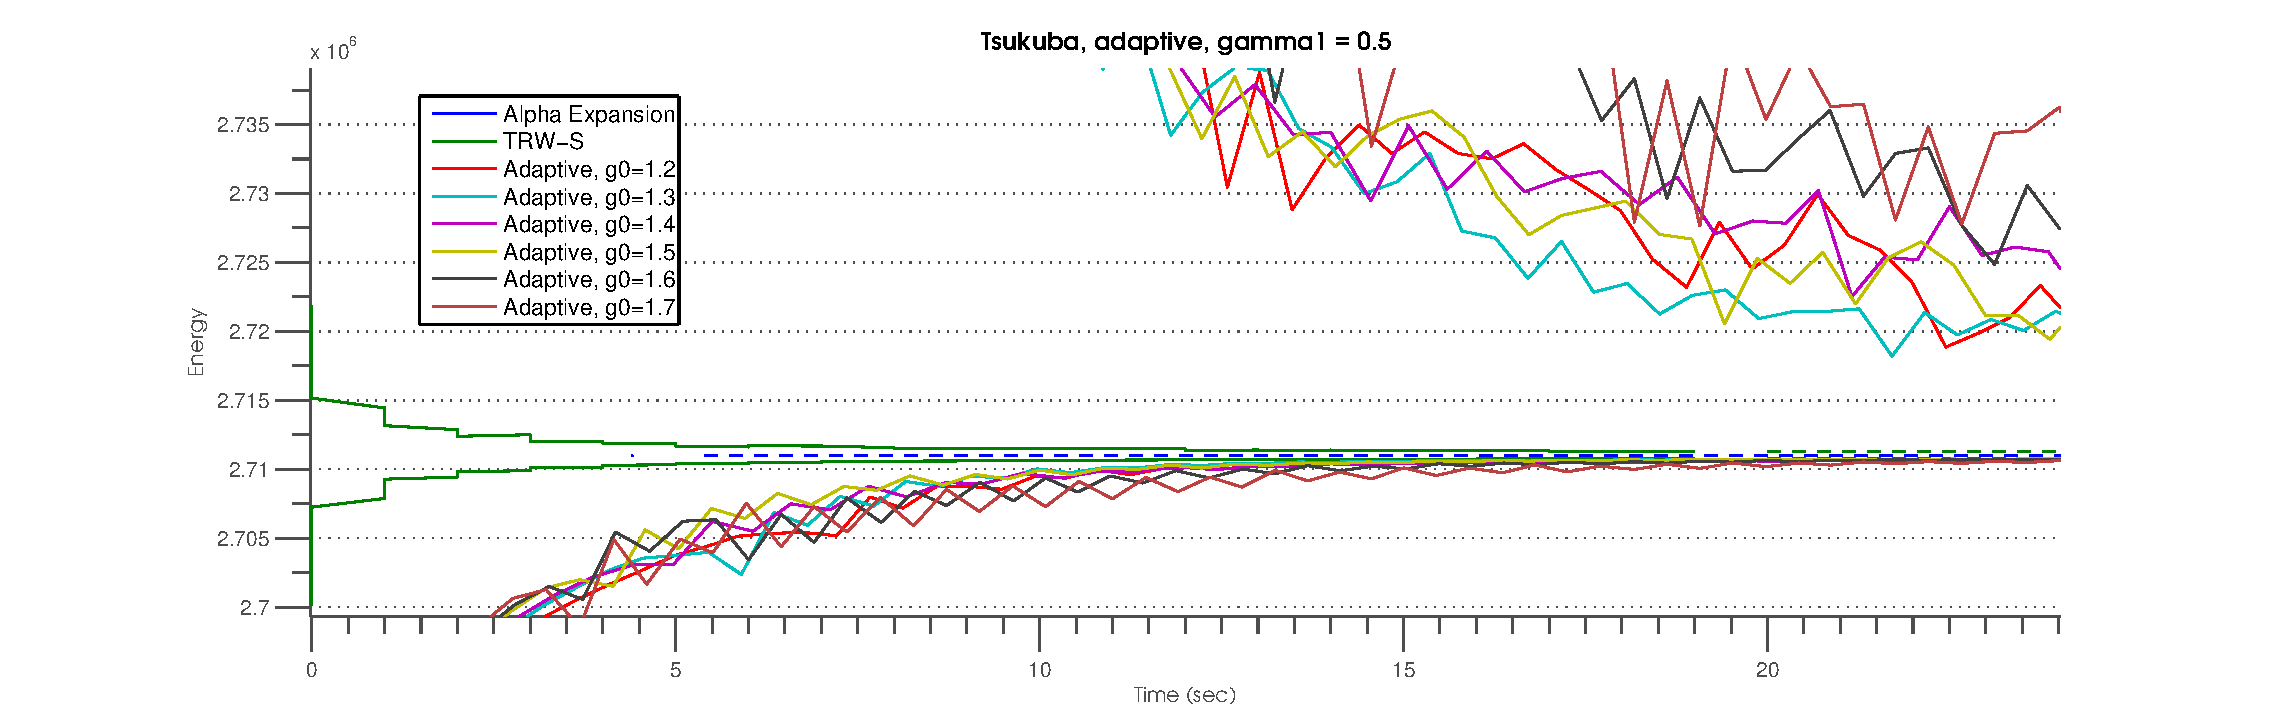
\includegraphics[scale=0.4]{adaptive_g0_tsukuba.eps}
    \end{figure}
\end{frame}

\begin{frame}
  \frametitle{Субградиентный подъем}
  \framesubtitle{Адаптивный выбор шага ($\gamma_1$)}
    \begin{figure}
      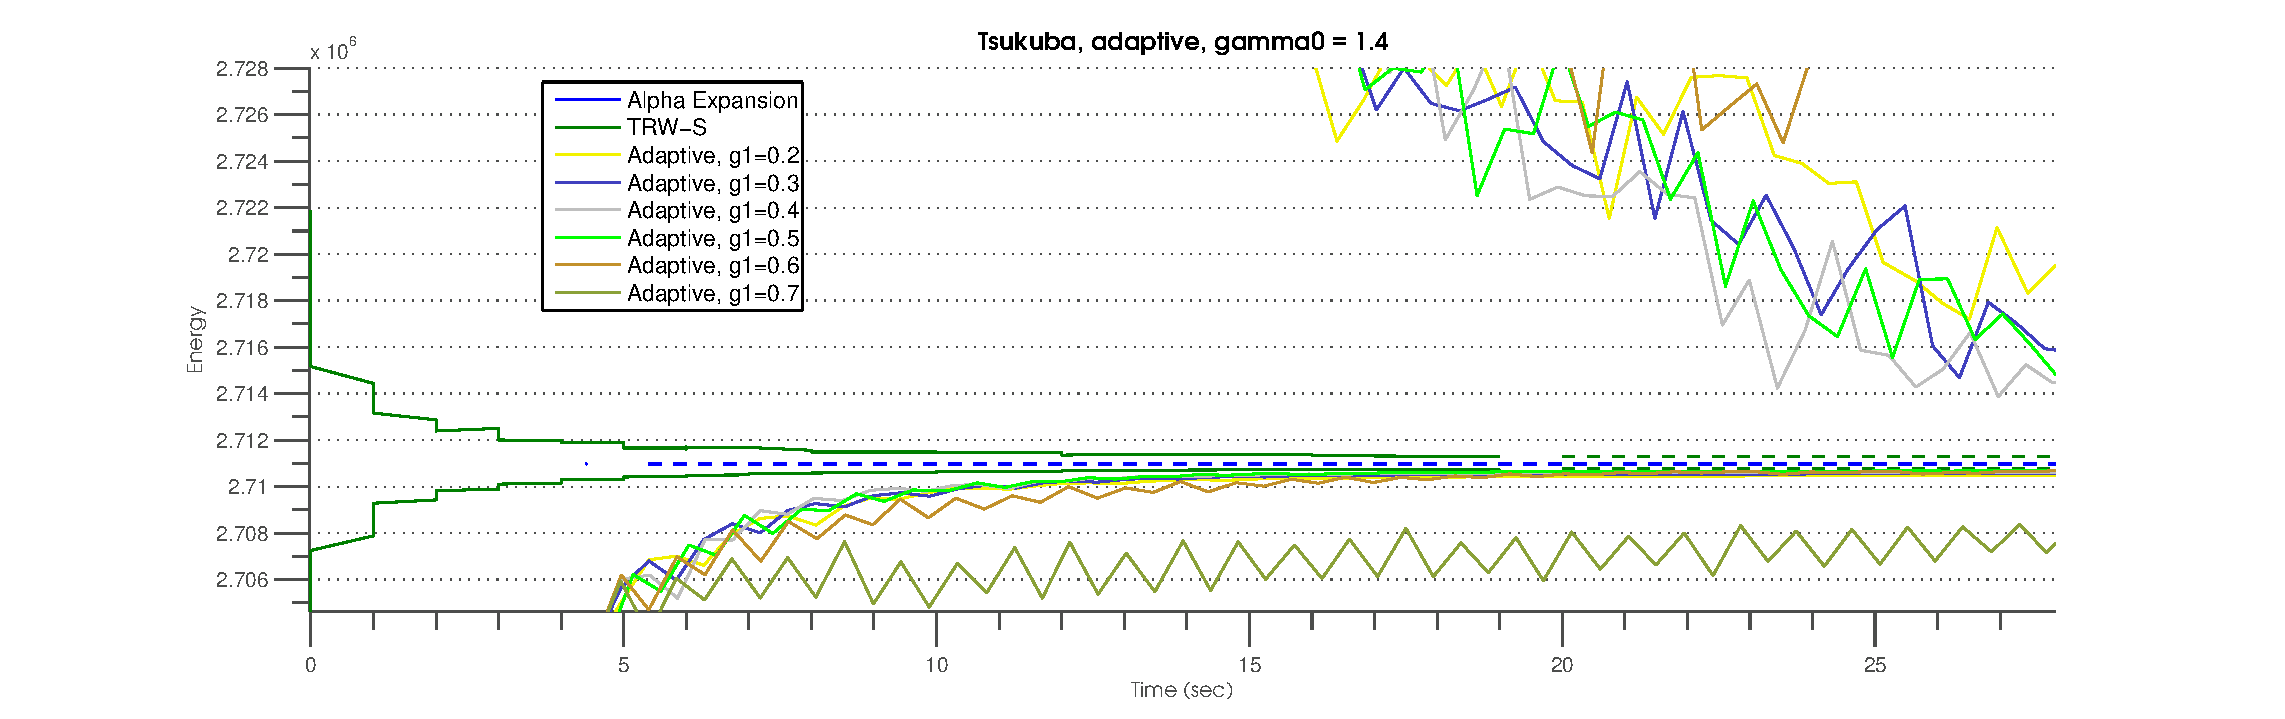
\includegraphics[scale=0.4]{adaptive_g1_tsukuba.eps}
    \end{figure}
\end{frame}

\begin{frame}
  \frametitle{Субградиентный подъем}
  \framesubtitle{Сравнение подходов}
  Обратите внимание на то, что по оси X отложенны внешние итерации метода.
    \begin{figure}
      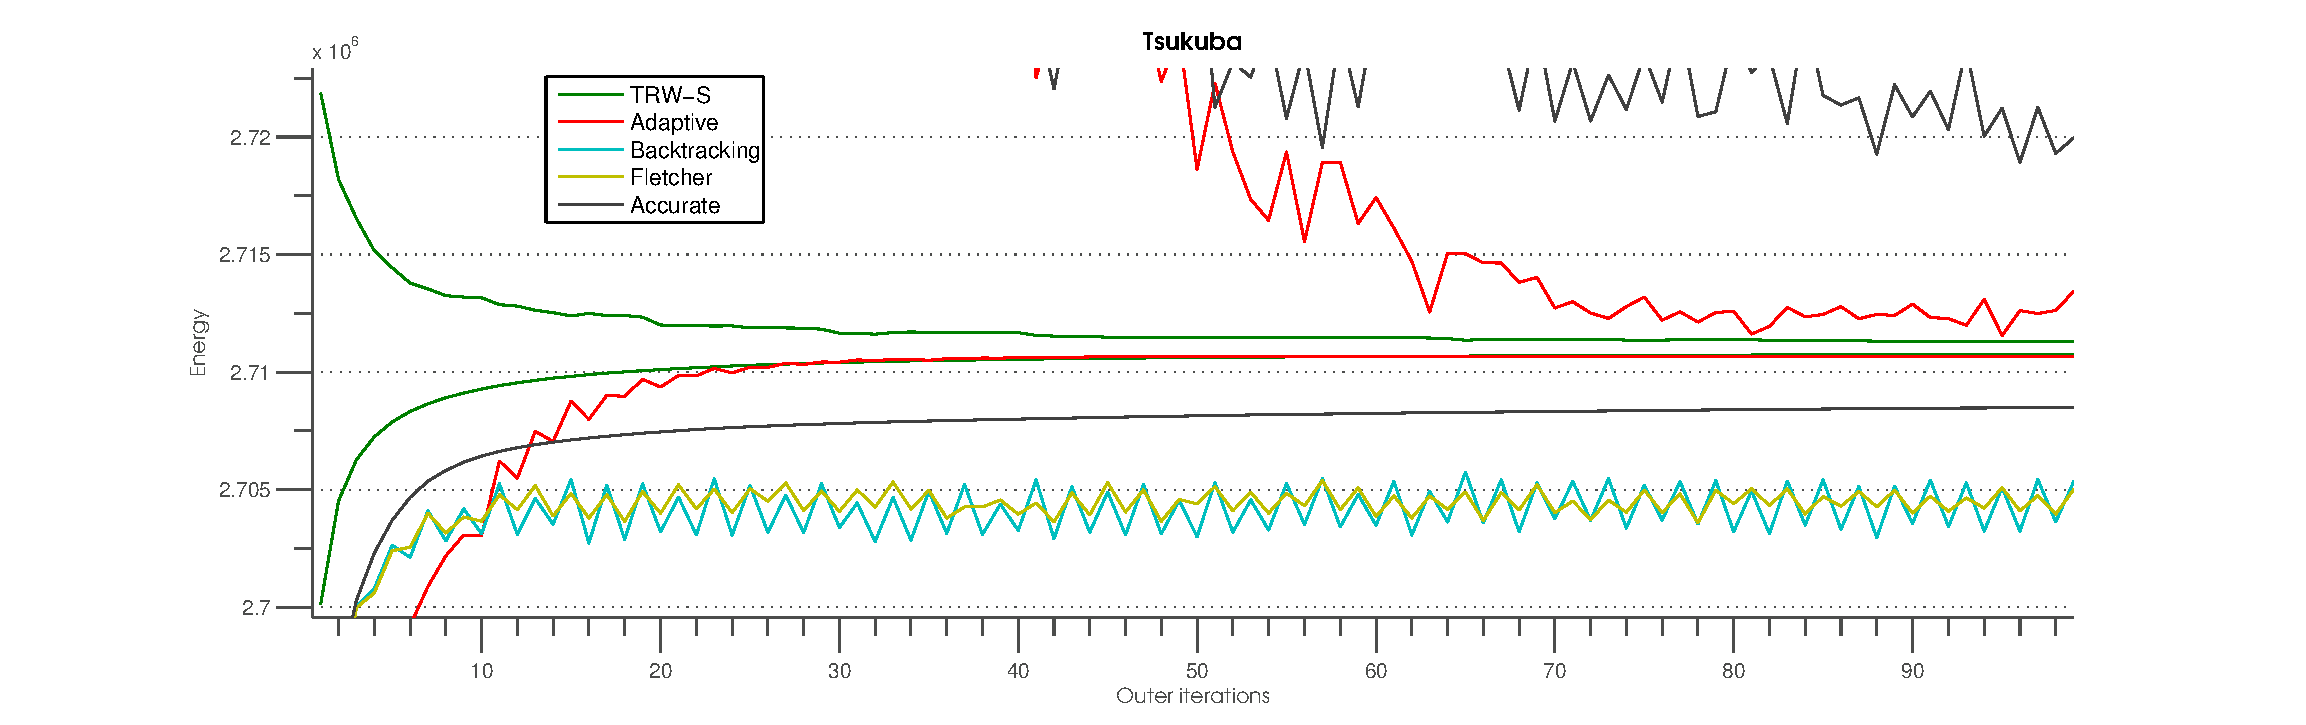
\includegraphics[scale=0.3]{subgradient_tsukuba.eps}
    \end{figure}
\end{frame}

\section{Bundle методы}
\begin{frame}
  \frametitle{Bundle approach}
  Построим простую глобальную оценку сверху и будем оптимизировать её:
    \begin{equation}
      \hat{f}(\lambda) = \min_{(\lambda{}', f(\lambda{}'), g{}') \in \mathcal{B}} \{f(\lambda{}') + <g{}', \lambda - \lambda{}'>\}
    \end{equation}
    \begin{equation}
      \lambda^{k + 1} = arg\max_{\lambda} \{\hat{f}(\lambda)  - \frac{w^k}{2} \left \| \lambda - \overline{\lambda} \right \|_2^2\}
    \end{equation}
    Качество работы алгоритма зависит от управления размером бандла и выбора весов. Авторы метода предлагают следующую формулу пересчета весов~\cite{Bundle}:
    \begin{equation}
       w^k = P_{[w_{min}, w_{max}]} \left ( \left (\gamma \cdot \frac{\min_{k}Upper^k - \max_{k} Dual^k}{\left \| P_{\mathcal{L}} ({g^k}) \right \|} \right )^{-1}\right )
    \end{equation}
\end{frame}

\begin{frame}
  \frametitle{Bundle approach, пример 1}
    Рассмотрим вариант с весом равным довольно большой константе 3.
    \begin{figure}
      \centering
      \begin{subfigure}[b]{0.45\textwidth}
              \centering
              \includegraphics[width=\textwidth]{bundle_example_1}
      \end{subfigure}%
      ~ %add desired spacing between images, e. g. ~, \quad, \qquad etc.
        %(or a blank line to force the subfigure onto a new line)
      \begin{subfigure}[b]{0.45\textwidth}
              \centering
              \includegraphics[width=\textwidth]{bundle_example_2}
      \end{subfigure}\\
      \begin{subfigure}[b]{0.45\textwidth}
              \centering
              \includegraphics[width=\textwidth]{bundle_example_3}
      \end{subfigure}
    \end{figure}
\end{frame}

\begin{frame}
  \frametitle{Bundle approach, пример 2}
    Теперь весом будет маленькая константа 0.7 и шаги увеличатся.
    \begin{figure}
      \centering
      \begin{subfigure}[b]{0.45\textwidth}
              \centering
              \includegraphics[width=\textwidth]{bundle_big_step_example_1}
      \end{subfigure}%
      ~ %add desired spacing between images, e. g. ~, \quad, \qquad etc.
        %(or a blank line to force the subfigure onto a new line)
      \begin{subfigure}[b]{0.45\textwidth}
              \centering
              \includegraphics[width=\textwidth]{bundle_big_step_example_2}
      \end{subfigure}\\
      \begin{subfigure}[b]{0.45\textwidth}
              \centering
              \includegraphics[width=\textwidth]{bundle_big_step_example_3}
      \end{subfigure}%
      ~ %add desired spacing between images, e. g. ~, \quad, \qquad etc.
        %(or a blank line to force the subfigure onto a new line)
      \begin{subfigure}[b]{0.45\textwidth}
              \centering
              \includegraphics[width=\textwidth]{bundle_big_step_example_4}
      \end{subfigure}
    \end{figure}
\end{frame}

\begin{frame}
  \frametitle{Bundle approach}
  Воспользуемся формулой от авторов и поварьируем размер бандла. При этом $w^k$ становится порядка $0.01$.
    \begin{figure}
      \includegraphics[scale=0.3]{bundle_natural_tsukuba_.eps}
    \end{figure}
\end{frame}


\begin{frame}
  \frametitle{Bundle approach}
  Теперь зафиксируем вес $w^k$ огромной константой (размер бандла = 10).
    \begin{figure}
      \includegraphics[scale=0.3]{bundle_const_w_tsukuba.eps}
    \end{figure}
\end{frame}

\section{Сравнение методов}
\begin{frame}
  \frametitle{Сравнение методов}
    \begin{figure}
      \includegraphics[scale=0.3]{comparison_tsukuba.eps}
    \end{figure}
\end{frame}

\begin{frame}
  \frametitle{Сравнение методов}
    \begin{figure}
      \includegraphics[scale=0.3]{comparison_tsukuba_big.eps}
    \end{figure}
\end{frame}

\section{Сравнение методов}
\begin{frame}
  \frametitle{Сравнение методов}
    Для стерео пары venus:
    \begin{figure}
      \includegraphics[scale=0.3]{comparison_venus.eps}
    \end{figure}
\end{frame}

\section{Выводы}
\begin{frame}
  \frametitle{Выводы, вклад}
  \begin{itemize}
    \item Реализован фреймворк для сравнения алгоритмов вывода в MRF
    \item Лучше всего работают aggregate bundle методы, тема ещё не до конца закончена (проблемы с выбором шага)
    \item На удивленее неплохо работает метод адаптивного субградиента
  \end{itemize}
\end{frame}


\begin{thebibliography}{1}
\bibitem{TRWS}
    {Kolmogorov~V.}
    {Convergent Tree-Reweighted Message Passing for Energy Minimization}~//
    {IEEE} Trans. Pattern Anal. Mach. Intell., 2006.~--- С.\,1568--1583.
\bibitem{ABundle}
    {Kiwiel~K.}
    {An aggregate subgradient method for nonsmooth convex minimization}~//
    Mathematical Programming, 1983, 27:320--341.
\bibitem{Alahari}
    {Alahari~K., Kohli~P., Torr~P.~H.~S.}
    {Dynamic Hybrid Algorithms for MAP Inference in Discrete MRFs}~//
    {IEEE} Trans. Pattern Anal. Mach. Intell., 2010.~--- С.\,1846--1857.
\bibitem{Subgradient}
    {Komodakis~N., Paragios~N., Tziritas~G.}
    {MRF energy minimization and beyond via dual decomposition}~//
    Pattern Analysis and Machine Intelligence, IEEE Transactions on, 2011.~--- С.\,531--552.
\bibitem{Bundle}
    {Kappes~J.\,H., Bogdan~Savchynskyy, Christoph~Schnorr}
    {A Bundle Approach To Efficient MAP-Inference by Lagrangian Relaxation}~//
    Computer Vision and Pattern Recognition (CVPR), IEEE Conference 2012.~--- С.\,1688--1695.
\end{thebibliography}
\end{document}
